%!TEX root =  ../main.tex

\subsection{Pecking Order}

\objective{Build and decompose a composition of functions and their derivatives.}


In elementary school, we learned that a mathematics sentence has a 
certain order of operations, that somethings must happen before others.
If we want to add before we multiply, we must notate parentheses,
because normally multiplication is repeated addition, something of a higher
order than simple addition.  These parentheses lead to a phenomenon
in mathematics that is difficult and unnatural, compared to all other
languages: inside to outside reading.

For example, in the function $f(x)=\frac{2(x^2+1)}{3}$, you know to follow a
sequence of operations on any given input:
\begin{itemize}
\item square it
\item add 1
\item multiply by two
\item divide by three
\end{itemize}
Natural language does something like this, but it is quite confusing to read
(try saying it aloud to yourself): I saw the child the man my girl hates fathered.
It might be better to make this entirely left-branching: I saw the child who
the man fathered who my girl hates!

Our example utilizes only elementary functions: squaring, adding, multiplying,
and dividing.  If we want to use arbitrary functions, we must write
$f(g(h(x)))$ or $(f\circ g\circ h)(x)$.

\subsection{Domain and Range}
Taking a function as a composition of two other (e.g. $f(x)=g(h(x))$), we observe
a ``chain'' of inputs to outputs.  This might be compared to the game of telephone,
where your ear receives a message from the person before you, garbles it in your
brain, and then outputs a transformed version from your mouth, to the next person's
ear.  In math, there is a domain for $h(x)$, a set of numbers it can take for input.
These numbers are mapped onto a range of outputs, which are then fed into
$g(x)$.  Now $g(x)$ had its own domain, and the output from $h$ is a subset of that
absolute domain.  Having received some input from a portion of its domain,
$h(x)$, now outputs a unique range.

\begin{figure}
\begin{center}
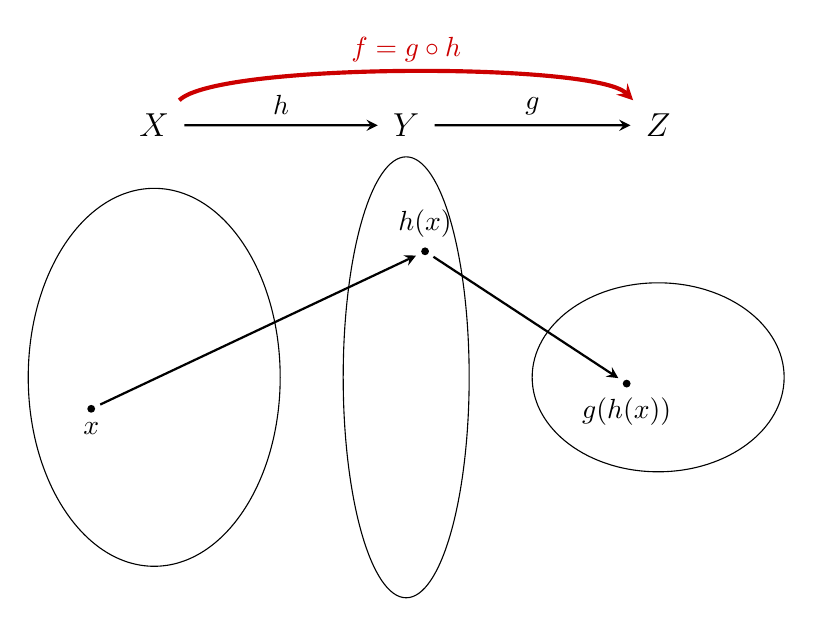
\begin{tikzpicture}[scale=0.8,
      >=stealth,
      bullet/.style={
        fill=black,
        circle,
        inner sep=1pt
      },
      projection/.style={
        ->,
        thick,
        shorten <=2pt,
        shorten >=2pt
      },
    ]

    \draw (0, 0) circle [x radius=2, y radius=3];
    \node [bullet, label=below:\(x\)] (x) at (-1, -0.5) {};
    \node[font=\large] (X) at (0, 4) {\(X\)};

    \begin{scope}[xshift=4cm]
      \draw (0, 0) circle [x radius=1, y radius=3.5]; \node [bullet,
      label=above:\(h(x)\)] (fx) at (0.3, 2) {};
      \node[font=\large] (Y) at (0, 4) {\(Y\)};
    \end{scope}
    \begin{scope}[xshift=8cm]
      \draw (0, 0) circle [x radius=2, y radius=1.5]; \node [bullet,
      label=below:\(g(h(x))\)] (gfx) at (-0.5, -0.1) {};
      \node[font=\large] (Z) at (0, 4) {\(Z\)};
    \end{scope}

    \draw [projection] (x) -- (fx);
    \draw [projection] (fx) -- (gfx);
    \draw [projection] (X) -- (Y)
          node [pos=0.5, above] {\(h\)};
    \draw [projection] (Y) -- (Z)
          node [pos=0.5, above] {\(g\)};
    \draw [out=45, in=180-45, projection, line width=1.5pt, red!80!black] 
          (X) .. controls ++(1, 1) and ++(-1, 1) .. (Z)
          node [pos=0.5, above] {\(f = g \circ h\)};
\end{tikzpicture}
\caption{Composition of functions \cite{sxtikzcomp}.}
\end{center}
\end{figure}
  
\subsection{Decomposition}
Any function with more than one operation can be written as the composition of
other functions.  For example, if $f(x)=x^2+1$ then we could construct
functions $g(x)=x^2$ and $h(x)=x+1$ such that $f(x)=h(g(x))$ ($g(h(x))$ would be
$(x+1)^2$).

\subsection{The Chain Rule}\index{derivative!chain rule}
The algebra of functions continues, even into the realm of derivatives.  Two functions
added would have a simple derivative: the sum of their respective derivatives.  But what 
of two functions composed?  What is the derivative of $g(h(x))$?

Here, Leibniz's notation is more helpful:

$$f(x)=g(h(x)), \quad \frac{df}{dx}=\frac{dg}{dh}\cdot\frac{dh}{dx}$$

\paragraph{Trigonometric Derivatives}\index{derivative!of sine}
While you are not responsible for proving and understanding trigonometric functions
until Part~\ref{pt:trig}, it is helpful to being memorizing facts about them now.  This will allow
you to practice manipulating the functions like any other.  However, to do so, you will
need to know the derivative of sine and cosine.\index{derivative!of cosine}

\begin{itemize}
\item $f(x) = \sin(x)$
\item $f'(x) = \cos(x)$
\item $f''(x) = -\sin(x)$
\item $f'''(x) = -\cos(x)$
\item $f^{(4)}(x) = \sin(x)$
\end{itemize}
As you can see, a straightforward, four-step cycle emerges.  The derivative of sine is
cosine.  The derivative of cosine is negative sine.


